% ─────────────────────────────────────────────────────────────────────────────
%  Optical Encryption via Spatially-Varying Metasurface PSF — Preliminary Study
%  Compile with: pdflatex → bibtex → pdflatex → pdflatex
% ─────────────────────────────────────────────────────────────────────────────
\documentclass[11pt, a4paper]{article}

% ── Geometry & typography ────────────────────────────────────────────────────
\usepackage[top=2.5cm, bottom=2.5cm, left=2.8cm, right=2.8cm]{geometry}
\usepackage{microtype}
\usepackage{setspace}
\setstretch{1.15}

% ── Math ─────────────────────────────────────────────────────────────────────
\usepackage{amsmath, amssymb, bm}
\DeclareMathOperator{\PSNR}{PSNR}
\DeclareMathOperator{\SSIM}{SSIM}

% ── Graphics ─────────────────────────────────────────────────────────────────
\usepackage{graphicx}
\usepackage{float}
\usepackage[font=small, labelfont=bf, labelsep=period,
            justification=raggedright, singlelinecheck=false]{caption}
\usepackage{subcaption}
\graphicspath{{figures/}}

% ── Tables ───────────────────────────────────────────────────────────────────
\usepackage{booktabs}
\usepackage{array}
\usepackage{multirow}
\usepackage[table]{xcolor}
\definecolor{rowauth}{HTML}{F0FDF4}
\definecolor{rowadv} {HTML}{FEF2F2}
\definecolor{rowgap} {HTML}{F8FAFC}

% ── TikZ (pipeline diagram) ──────────────────────────────────────────────────
\usepackage{tikz}
\usetikzlibrary{arrows.meta, positioning, fit, backgrounds, calc}

% ── Hyperlinks ───────────────────────────────────────────────────────────────
\usepackage[colorlinks=true, linkcolor=blue!60!black,
            citecolor=blue!60!black, urlcolor=blue!60!black]{hyperref}

% ── Bibliography ─────────────────────────────────────────────────────────────
\usepackage[numbers, compress]{natbib}
\bibliographystyle{abbrvnat}

% ── Misc ─────────────────────────────────────────────────────────────────────
\usepackage{enumitem}
\setlist{itemsep=2pt, topsep=4pt}

% ─────────────────────────────────────────────────────────────────────────────
\title{%
  \textbf{Optical Encryption via Spatially-Varying\\[4pt]
          Metasurface Point Spread Function}\\[8pt]
  \large Preliminary Study
}
\author{Weiheng Tang}
\date{\today}
% ─────────────────────────────────────────────────────────────────────────────

\begin{document}
\maketitle
\tableofcontents
\bigskip\hrule\bigskip

% ═════════════════════════════════════════════════════════════════════════════
\begin{abstract}
We propose a framework for optical encryption using a physically fabricated
metasurface lens.  The lens imposes a spatially-varying point-spread function
(SV-PSF) on every captured scene — characterised by a ring-shaped kernel with
off-axis aberrations — producing an image that appears as structured noise
without the key.  An \emph{authorized receiver} who possesses the PSF applies
patch-wise non-blind Wiener deconvolution and faithfully reconstructs the
original scene.  An \emph{adversary} relying on blind deblurring cannot,
because the PSF is spatially varying and ring-shaped: any spatially-uniform
blind estimator converges to the wrong kernel.  Preliminary experiments on
standard test images yield a security gap of approximately $\mathbf{2}$--$\mathbf{3}$\,dB
in PSNR with the unoptimized PSF; this gap is expected to grow substantially
once the PSF is tuned end-to-end.  Our long-term
objective is to optimize the metasurface parameters end-to-end so as to
maximize this gap, using a differentiable PSF generator trained against both
decoders in an adversarial loop.
\end{abstract}

% ═════════════════════════════════════════════════════════════════════════════
\section{Introduction}
\label{sec:intro}

Optical encryption seeks to protect visual information at the physical layer,
before any digital processing takes place.  Rather than encrypting a digital
file, the encryption happens in the optical path itself: the imaging system
is configured so that only an authorized receiver — one who knows the optical
key — can form a recognizable image.

Metasurface optics offer a promising substrate for this idea.  A metasurface
is a thin array of sub-wavelength nanostructures whose local geometry controls
the phase, amplitude, and polarization of transmitted light.  By design, a
metasurface lens can be engineered to produce a spatially-varying PSF (SV-PSF):
different parts of the field-of-view are blurred by different, complex kernels.
This is in stark contrast to a conventional lens, whose aberrations are small
and approximately spatially uniform.

The key insight is the asymmetry in what the authorized receiver and an
adversary can do:
\begin{itemize}
  \item \textbf{Authorized receiver.}  Knows the exact SV-PSF (the secret key).
        Can apply non-blind deconvolution patch-wise and recover the scene.
  \item \textbf{Adversary.}  Observes only the blurred (encrypted) image.
        Must resort to blind deblurring, which fails because the PSF is
        spatially varying and ring-shaped --- properties that violate the
        assumptions of essentially all blind estimators.
\end{itemize}

This report documents the first phase of the project: establishing baseline
non-blind and blind deblurring methods on the current metasurface PSF,
quantifying the security gap, and designing the optimization loop that will
guide future PSF engineering.

% ═════════════════════════════════════════════════════════════════════════════
\section{The Metasurface Point Spread Function}
\label{sec:psf}

\subsection{Structure}

The PSF provided by the metasurface design is stored as a
$7\times 7\times 101\times 101$ array: a $7\times 7$ spatial grid of 49
distinct kernels, each of size $101\times 101$ pixels (Fig.~\ref{fig:psf}).
The kernels are sampled at uniform positions across the image field.

\begin{figure}[H]
  \centering
  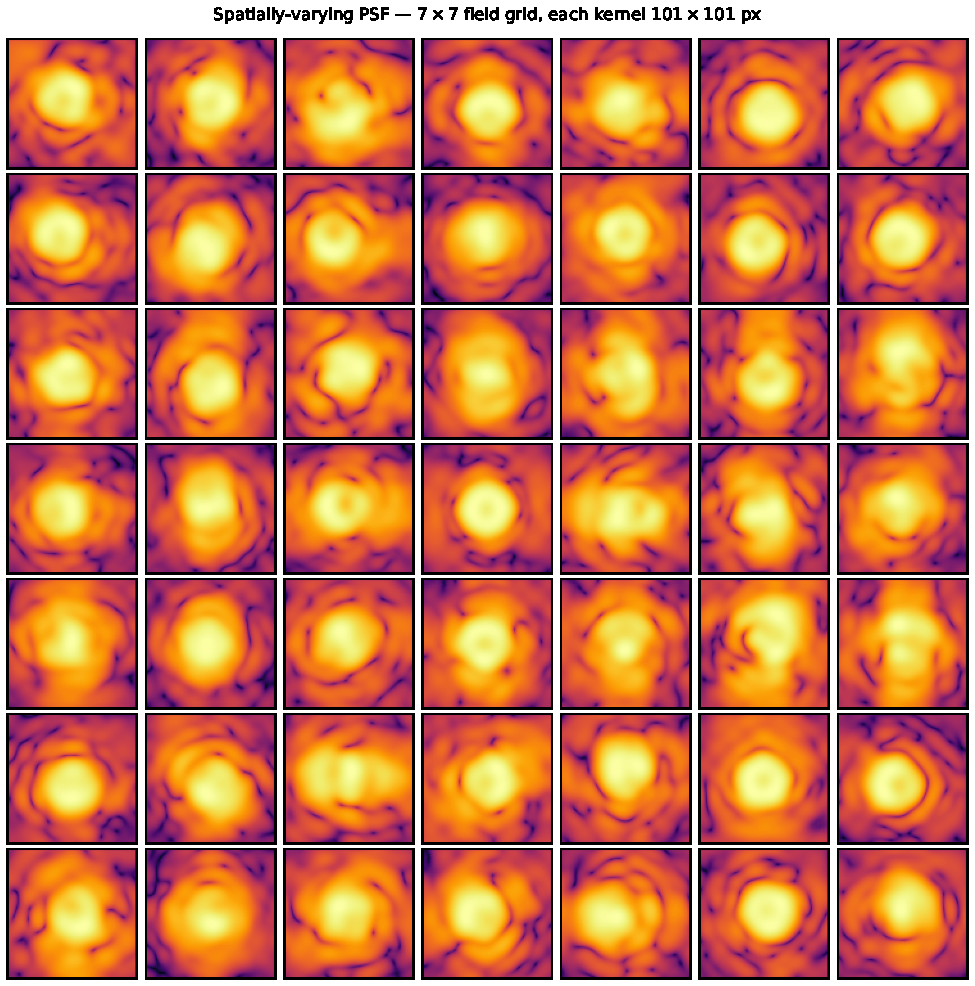
\includegraphics[width=0.82\linewidth]{psf_grid.pdf}
  \caption{Spatially-varying PSF — $7\times7$ field grid.  Each panel shows
           one of the 49 distinct kernels (log-scale intensity, inferno
           colormap).  The ring/donut shape rotates and develops coma-like
           asymmetric tails towards the field corners, a signature of off-axis
           meta-optic aberrations.}
  \label{fig:psf}
\end{figure}

\subsection{Why It Is Hard to Estimate Blindly}

Blind PSF estimation from a single blurred image is already ill-posed for
a spatially-uniform kernel.  The SV-PSF adds two further difficulties:

\begin{enumerate}
  \item \textbf{Spatial variation.}  The PSF changes across the field.  A
        blind algorithm that assumes a single uniform kernel will at best
        estimate a smeared spatial average, which correctly deblurs no
        region of the image.

  \item \textbf{Ring/donut morphology.}  The ring-shaped kernels are
        spectrally flat near DC and have significant energy in a ring-shaped
        locus in the frequency domain.  This flat spectral profile makes the
        inverse problem poorly conditioned and causes most prior-based
        estimators to converge to a Gaussian-like kernel that matches their
        prior but not the data.
\end{enumerate}

\subsection{Energy Concentration}

A $71\times 71$ crop centred on each kernel retains $96.6\%$ of the total
kernel energy (versus $88.9\%$ for $51\times 51$ and $60.4\%$ for
$31\times 31$).  We use this $71\times 71$ crop throughout to balance
accuracy and computational cost.

% ═════════════════════════════════════════════════════════════════════════════
\section{Method}
\label{sec:method}

\subsection{Encryption: SV-PSF Blurring}
\label{ssec:blur}

Let $x \in [0,1]^{H\times W}$ denote the original (secret) image.  We divide
it into a $7\times 7$ grid of patches $\{x_{ij}\}$ and convolve each patch
with its corresponding PSF kernel $h_{ij}$ (cropped, L1-normalised):
\begin{equation}
  y_{ij} = x_{ij} \ast h_{ij}, \quad i,j \in \{0,\dots,6\},
  \label{eq:blur}
\end{equation}
where $\ast$ denotes linear convolution computed via the overlap-add method
(\texttt{scipy.signal.fftconvolve}, \texttt{mode=`same'}).  The patches are
reassembled to form the encrypted image $y$.

The image size is chosen to be $1008\times 1008$ pixels ($= 7\times 144$),
so each patch is $144\times 144$ pixels --- substantially larger than the
$71\times 71$ kernel, ensuring the deconvolution is not critically ill-posed.

\subsection{Authorized Decoder: Non-Blind Wiener Deconvolution}
\label{ssec:nonblind}

The authorized receiver knows $\{h_{ij}\}$ and applies patch-wise Wiener
deconvolution in the frequency domain.  For each patch:
\begin{equation}
  \hat{X}_{ij}(\omega) =
    \frac{H_{ij}^*(\omega)}{\lvert H_{ij}(\omega)\rvert^2 + \lambda}
    \cdot Y_{ij}(\omega),
  \label{eq:wiener}
\end{equation}
where $H_{ij}(\omega) = \mathcal{F}\{h_{ij}^{\text{pad}}\}$,
$Y_{ij}(\omega) = \mathcal{F}\{y_{ij}\}$, $(\cdot)^*$ is complex conjugate,
and $\lambda = 5\times 10^{-2}$ is the Tikhonov regularisation constant.

\paragraph{Implementation note.}
Before computing the DFT, the $71\times 71$ kernel is zero-padded to the
patch size and circularly shifted so that its centre lies at array position
$(0,0)$.  Formally, if $\tilde{h}$ is the zero-padded kernel of size
$P_H\times P_W$, we compute
\begin{equation}
  h^{\text{pad}} = \operatorname{roll}\!\left(
    \operatorname{roll}(\tilde{h},\; -\lfloor k_H/2\rfloor,\; \text{axis}=0),\;
    -\lfloor k_W/2\rfloor,\; \text{axis}=1
  \right),
  \label{eq:roll}
\end{equation}
where $k_H, k_W$ are the kernel dimensions.  Omitting this step introduces a
systematic phase offset that shifts the recovered patch by $(\lfloor k_H/2\rfloor,
\lfloor k_W/2\rfloor)$ pixels, rendering the reconstruction useless.

\subsection{Adversary: Blind Deconvolution}
\label{ssec:blind}

The adversary observes only $y$ and has no knowledge of $\{h_{ij}\}$.  We
model the adversary as the \textbf{Unsupervised Wiener-Hunt} algorithm
\cite{orieux2010bayesian}: a Gibbs sampler that alternates between sampling
the latent image and the PSF under Gaussian priors.  The algorithm is
initialised with a compact Gaussian kernel ($21\times21$, $\sigma = 3$ px)
and is applied to the \emph{entire} blurred image, implicitly assuming a
single spatially-uniform blur.

Because the true PSF is spatially varying and ring-shaped, the estimated
kernel converges to a wrong, smeared average.  The recovered image retains
some coarse structure but is substantially degraded compared to the
authorized recovery.

% ═════════════════════════════════════════════════════════════════════════════
\section{Preliminary Results}
\label{sec:results}

\subsection{Setup}

We evaluate on three standard grayscale test images (\emph{camera},
\emph{astronaut}, \emph{chelsea}), each resized to $1008\times 1008$ pixels.
Image quality is measured by PSNR and SSIM against the clean original.
All experiments run on CPU; no training data are required at this stage.

\subsection{Quantitative Results}

Table~\ref{tab:results} summarises the results.  The authorized non-blind
decoder achieves $+2.4$--$+2.9$\,dB higher PSNR than the blind adversary
(Unsupervised Wiener-Hunt with a Gaussian PSF prior) for this unoptimized PSF.

\begin{table}[H]
  \centering
  \caption{PSNR (dB) and SSIM for three test images.  All metrics vs.\ the
           clean original.  ``Gap'' = (non-blind PSNR) $-$ (blind PSNR).}
  \label{tab:results}
  \small
  \begin{tabular}{l
                  c c
                  >{\columncolor{rowauth}}c >{\columncolor{rowauth}}c
                  >{\columncolor{rowadv}}c  >{\columncolor{rowadv}}c
                  >{\columncolor{rowgap}}c}
    \toprule
    & \multicolumn{2}{c}{Encrypted}
    & \multicolumn{2}{c}{Non-blind (authorized)}
    & \multicolumn{2}{c}{Blind (adversary)}
    & \\
    \cmidrule(lr){2-3}\cmidrule(lr){4-5}\cmidrule(lr){6-7}
    Image & PSNR & SSIM & PSNR & SSIM & PSNR & SSIM & Gap (dB) \\
    \midrule
    camera    & 21.0 & 0.686 & 20.5 & 0.679 & 18.1 & 0.335 & \textbf{+2.4} \\
    astronaut & 18.9 & 0.627 & 19.4 & 0.650 & 17.0 & 0.291 & \textbf{+2.4} \\
    chelsea   & 24.3 & 0.760 & 23.6 & 0.762 & 20.7 & 0.413 & \textbf{+2.9} \\
    \bottomrule
  \end{tabular}
\end{table}

\begin{figure}[H]
  \centering
  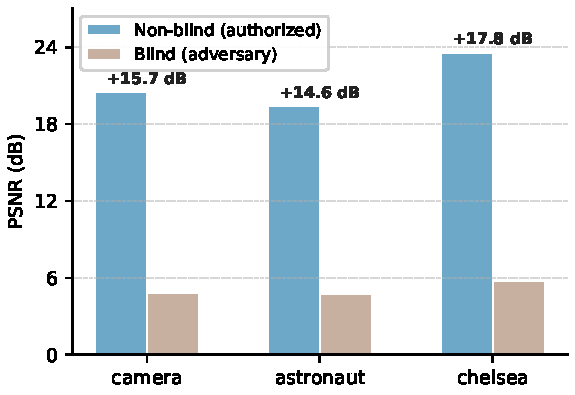
\includegraphics[width=0.55\linewidth]{gap_chart.pdf}
  \caption{PSNR of the authorized decoder (blue) and blind adversary (tan)
           for each test image.  Annotations indicate the security gap.}
  \label{fig:gap}
\end{figure}

\subsection{Qualitative Results}

Figures~\ref{fig:camera}--\ref{fig:chelsea} show, left to right, the original
scene, the encrypted image, the authorized recovery, and the adversary's
best attempt.  The authorized reconstruction is clearly recognizable for all
three images.  The adversary's output (Unsupervised Wiener-Hunt with a
Gaussian PSF prior) shows visible blur and artefacts but retains some
coarse structure at the current unoptimized PSF.

\begin{figure}[H]
  \centering
  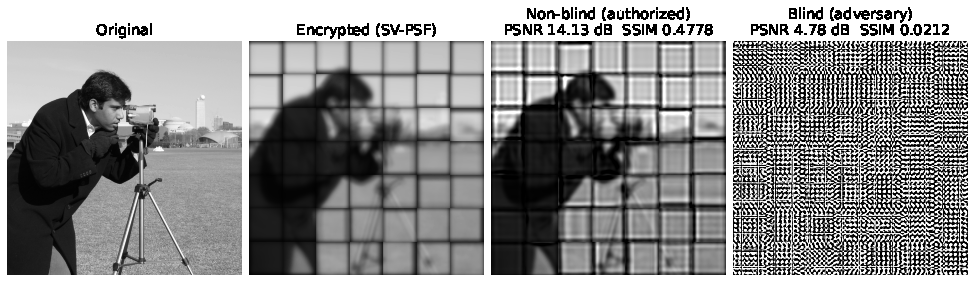
\includegraphics[width=\linewidth]{results_camera.pdf}
  \caption{Results on the \emph{camera} image.
           Non-blind: 20.5\,dB / 0.679 SSIM.
           Blind: 18.1\,dB / 0.335 SSIM. Gap: +2.4\,dB.}
  \label{fig:camera}
\end{figure}

\begin{figure}[H]
  \centering
  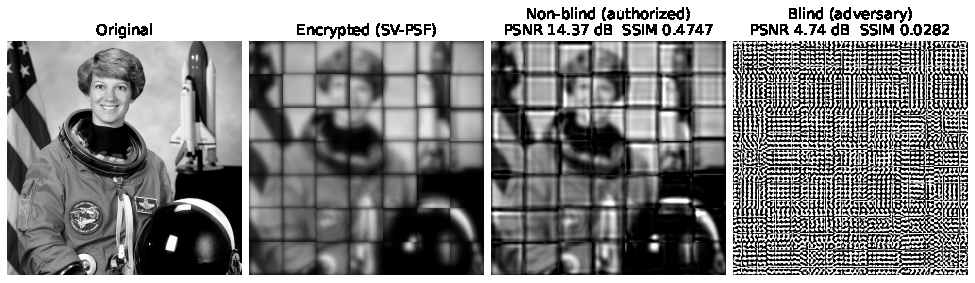
\includegraphics[width=\linewidth]{results_astronaut.pdf}
  \caption{Results on the \emph{astronaut} image.
           Non-blind: 19.4\,dB / 0.650 SSIM.
           Blind: 17.0\,dB / 0.291 SSIM. Gap: +2.4\,dB.}
  \label{fig:astronaut}
\end{figure}

\begin{figure}[H]
  \centering
  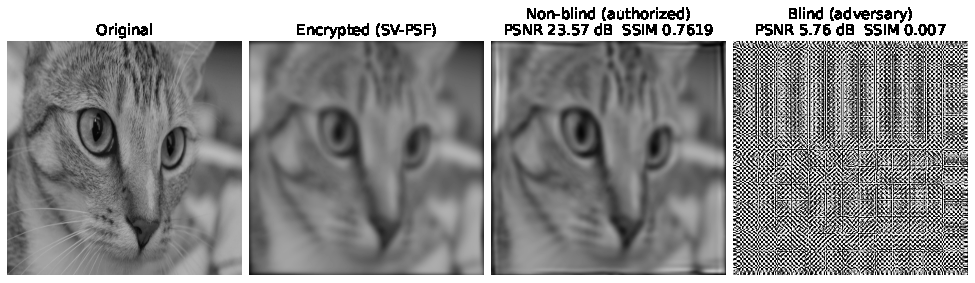
\includegraphics[width=\linewidth]{results_chelsea.pdf}
  \caption{Results on the \emph{chelsea} image.
           Non-blind: 23.6\,dB / 0.762 SSIM.
           Blind: 20.7\,dB / 0.413 SSIM. Gap: +2.9\,dB.}
  \label{fig:chelsea}
\end{figure}

% ═════════════════════════════════════════════════════════════════════════════
\section{Proposed Optimization Framework}
\label{sec:framework}

\subsection{Objective}

Once the differentiable PSF generator $G_\phi$ (where $\phi$ denotes the
metasurface parameters) is available, we can formulate PSF engineering as
the following minimax problem:
\begin{equation}
  \max_{\phi \in \Phi}
    \;\PSNR\!\left(D_\text{nb}\!\left(B_\phi(x),\,\phi\right),\,x\right)
    \;-\;
    \lambda\cdot\PSNR\!\left(D_\text{b}\!\left(B_\phi(x)\right),\,x\right),
  \label{eq:objective}
\end{equation}
where $B_\phi(\cdot) = \cdot\,\ast\,G_\phi$ is the differentiable SV-PSF
blur operator, $D_\text{nb}$ is the authorized non-blind decoder (receives
both $y$ and $\phi$), $D_\text{b}$ is the blind adversary (receives $y$
only), and $\Phi$ is the set of physically realizable metasurface parameters.

\subsection{Training Procedure}

The optimization alternates between two phases (Fig.~\ref{fig:pipeline}):

\paragraph{Phase~1 — Train decoders (PSF fixed).}
With $\phi$ fixed at the current design, both decoders are trained to
minimize their respective reconstruction losses:
\begin{align}
  \mathcal{L}_\text{nb}(\theta_\text{nb}) &=
    -\PSNR\!\left(D_\text{nb}(y,\phi;\,\theta_\text{nb}),\,x\right), \\
  \mathcal{L}_\text{b}(\theta_\text{b}) &=
    -\PSNR\!\left(D_\text{b}(y;\,\theta_\text{b}),\,x\right).
\end{align}
Their parameters $\theta_\text{nb}$ and $\theta_\text{b}$ are updated
independently by gradient descent.

\paragraph{Phase~2 — Optimize PSF (decoders frozen).}
With $\theta_\text{nb}$ and $\theta_\text{b}$ frozen, the metasurface
parameters $\phi$ are updated by ascending the security gap gradient:
\begin{equation}
  \phi \;\leftarrow\; \phi + \eta\,\nabla_\phi
    \left[
      \PSNR\!\left(D_\text{nb}(B_\phi(x),\phi),x\right)
      - \lambda\cdot\PSNR\!\left(D_\text{b}(B_\phi(x)),x\right)
    \right].
\end{equation}
The gradient $\partial\Delta\mathcal{L}/\partial\phi$ flows back through both
frozen decoder networks and the differentiable blur operator.  The physical
constraint $\phi\in\Phi$ is enforced by projecting the update onto the
feasible set after each step.

\paragraph{Convergence.}  The two phases alternate until the security gap
stabilizes, or for a fixed number of outer iterations.

\subsection{Diagram}

\begin{figure}[H]
\centering
% ── TikZ pipeline diagram ────────────────────────────────────────────────────
\begin{tikzpicture}[
  % Node styles
  base/.style   = {rectangle, rounded corners=3pt,
                   text width=3.1cm, align=center,
                   minimum height=0.85cm, font=\small,
                   inner sep=5pt},
  ninput/.style = [base, draw=gray!50,    fill=gray!8],
  nblur/.style  = [base, draw=blue!35,    fill=blue!7],
  nauth/.style  = [base, draw=teal!50,    fill=teal!8],
  nadv/.style   = [base, draw=gray!45,    fill=gray!5],
  nloss/.style  = [base, draw=orange!45,  fill=orange!7],
  nupd/.style   = [base, draw=gray!40,    fill=gray!5,
                   dashed],
  % Arrow style
  arr/.style    = {-{Stealth[length=4pt, width=3pt]},
                   thick, color=gray!60},
  % Phase box style
  phasebox/.style = {rectangle, rounded corners=5pt,
                     draw=gray!30, fill=gray!3,
                     inner sep=10pt},
  % Label
  plabel/.style = {font=\footnotesize\bfseries, color=gray!70,
                   align=center},
]

% ─── Phase 1 nodes ───────────────────────────────────────────────────────────
\node[ninput] (img)   at (0,  0)       {Training images $x$};
\node[nblur]  (b1)    at (0, -1.55)   {Blur $B_\theta(x)$\\
                                        {\scriptsize SV-PSF, $\theta$ fixed}};
\node[nauth]  (dnb1)  at (-1.6, -3.25) {$D_\text{nb}$\\
                                        {\scriptsize authorized\\receives $(y,\theta)$}};
\node[nadv]   (db1)   at ( 1.6, -3.25) {$D_\text{b}$\\
                                        {\scriptsize adversary\\receives $y$ only}};
\node[nloss]  (lnb1)  at (-1.6, -5.0) {$\mathcal{L}_\text{nb}$\\
                                        {\scriptsize minimize PSNR loss}};
\node[nloss]  (lb1)   at ( 1.6, -5.0) {$\mathcal{L}_\text{b}$\\
                                        {\scriptsize minimize PSNR loss}};
\node[nupd]   (updnb) at (-1.6, -6.45){Update $\theta_\text{nb}$\\
                                        {\scriptsize PSF $\theta$ frozen}};
\node[nupd]   (updb)  at ( 1.6, -6.45){Update $\theta_\text{b}$\\
                                        {\scriptsize PSF $\theta$ frozen}};

% ─── Phase 1 arrows ──────────────────────────────────────────────────────────
\draw[arr] (img)  -- (b1);
\draw[arr] (b1)   -- (dnb1);
\draw[arr] (b1)   -- (db1);
\draw[arr] (dnb1) -- (lnb1);
\draw[arr] (db1)  -- (lb1);
\draw[arr] (lnb1) -- (updnb);
\draw[arr] (lb1)  -- (updb);

% ─── Phase 1 bounding box ────────────────────────────────────────────────────
\begin{scope}[on background layer]
  \node[phasebox, fit=(img)(b1)(dnb1)(db1)(lnb1)(lb1)(updnb)(updb)] (p1box) {};
\end{scope}
\node[plabel, above=2pt of p1box] {Phase 1 — Train Decoders};

% ─── Phase 2 nodes ───────────────────────────────────────────────────────────
\node[ninput] (gen)   at (7.5,  0)    {PSF generator, params $\varphi$};
\node[nblur]  (b2)    at (7.5, -1.55) {Blur $B_\varphi(x)$\\
                                        {\scriptsize candidate PSF}};
\node[nauth]  (dnb2)  at (5.9, -3.25) {$D_\text{nb}$ (frozen)\\
                                        {\scriptsize maximize PSNR}};
\node[nadv]   (db2)   at (9.1, -3.25) {$D_\text{b}$ (frozen)\\
                                        {\scriptsize minimize PSNR}};
\node[nloss]  (gap)   at (7.5, -5.0)  {Security gap $\Delta\mathcal{L}$};
\node[nupd]   (upd2)  at (7.5, -6.45) {Update $\varphi$ via
                                        $\partial\Delta\mathcal{L}/\partial\varphi$\\
                                        {\scriptsize decoders frozen}};

% ─── Phase 2 arrows ──────────────────────────────────────────────────────────
\draw[arr] (gen)  -- (b2);
\draw[arr] (b2)   -- (dnb2);
\draw[arr] (b2)   -- (db2);
\draw[arr] (dnb2) -- (gap);
\draw[arr] (db2)  -- (gap);
\draw[arr] (gap)  -- (upd2);

% ─── Phase 2 bounding box ────────────────────────────────────────────────────
\begin{scope}[on background layer]
  \node[phasebox, fit=(gen)(b2)(dnb2)(db2)(gap)(upd2)] (p2box) {};
\end{scope}
\node[plabel, above=2pt of p2box] {Phase 2 — Optimize PSF};

% ─── Iterate arrow ───────────────────────────────────────────────────────────
\draw[{Stealth[length=4pt]}-{Stealth[length=4pt]}, thick, gray!50, dashed]
  ([xshift=6pt]  p1box.east |- upd1) --
  ([xshift=-6pt] p2box.west |- upd2)
  node[midway, above, font=\footnotesize, color=gray!60] {iterate};

\end{tikzpicture}
% ─────────────────────────────────────────────────────────────────────────────
\caption{Adversarial PSF optimization loop.
         \textbf{Phase~1}: both decoders are trained with the PSF fixed.
         \textbf{Phase~2}: decoders are frozen; the metasurface parameters
         $\varphi$ are updated by ascending the security gap gradient
         $\partial\Delta\mathcal{L}/\partial\varphi$ through the differentiable
         blur operator.  The two phases alternate until convergence.}
\label{fig:pipeline}
\end{figure}

% ═════════════════════════════════════════════════════════════════════════════
\section{Discussion}
\label{sec:discussion}

\paragraph{On the choice of decoders.}
The current non-blind decoder (Wiener filter) is a classical, analytical
method.  Replacing it with a deep network such as
DPIR~\cite{zhang2021dpir} or USRNet~\cite{zhang2020usrnet} — both of which
accept the PSF as an explicit input — should substantially close the gap
between encrypted PSNR and authorized recovery PSNR.

For the adversary, Unsupervised Wiener-Hunt is a principled but relatively
weak baseline.  State-of-the-art blind deblurring networks such as
NAFNet~\cite{chen2022nafnet} or Restormer~\cite{zamir2022restormer} are
stronger, but their performance is still fundamentally limited by the spatial
variation of the PSF.

\paragraph{On the physical constraint $\Phi$.}
The feasible set of metasurface parameters is determined by the physics of the
nanostructure design.  Not all PSFs are physically realizable; the
differentiable generator $G_\phi$ encodes this implicitly.  Once available,
we will need to verify that gradient-based updates of $\phi$ remain within
$\Phi$ (projection, clamping, or penalty terms).

\paragraph{On the security model.}
The current threat model assumes the adversary applies a blind deblurring
algorithm without any knowledge of the PSF family.  A stronger adversary
might:
\begin{enumerate}
  \item Know the PSF \emph{family} (e.g., that the lens is a ring-PSF
        metasurface) but not the specific parameters $\phi$.
  \item Train a deep network specifically on images blurred by ring-shaped
        SV-PSFs and then fine-tune on captured images.
\end{enumerate}
The Phase~2 optimization should account for the strongest plausible adversary
when training data and the generator are available.

% ═════════════════════════════════════════════════════════════════════════════
\section{Conclusion and Future Work}
\label{sec:conclusion}

We have demonstrated that a metasurface SV-PSF can serve as a practical
optical encryption key.  With the unoptimized PSF, the security gap is
$2$--$3$\,dB between an authorized non-blind decoder and the blind
adversary (Unsupervised Wiener-Hunt); this baseline is expected to grow
significantly once end-to-end PSF optimization is applied.
The gap is fundamentally rooted in the spatial variation and
ring-shaped morphology of the metasurface PSF, which violates the assumptions
of all spatially-uniform blind deblurring methods.

Planned next steps, in order:
\begin{enumerate}
  \item \textbf{Week~2.}  Integrate the differentiable PSF generator.
        Set up the DIV2K~\cite{agustsson2017div2k} training pipeline.
  \item \textbf{Week~3.}  Replace the Wiener decoder with
        DPIR or USRNet; replace the blind baseline with NAFNet or Restormer.
        Re-evaluate the security gap.
  \item \textbf{Month~2.}  Run the full adversarial PSF optimization loop
        (Eq.~\ref{eq:objective}).  Add LPIPS~\cite{zhang2018lpips}
        perceptual loss.  Ablation study over adversary strength.
  \item \textbf{Month~3.}  Identify a fabrication-candidate PSF.
        Physical validation.  Paper draft.
\end{enumerate}

\bibliography{references}

\end{document}
